\chapter{Line bundles}
\label{ch:line_bundles}

\section{Overview}

You might have heard about line bundles, which is somehow ``a set $L$ with a map $\pi \colon L \to
X$ where the preimage of each point is a line''.
And then, in the algebraic geometry section, you come across the concept of ``section'' which
appears to be just a function.

That sounds reasonable, but you may ask, ``so what? Isn't it then just another complex manifold
which has one more dimension than $X$? Why not just study complex manifold?''

It's true, but there are more structures on a line bundle:
\begin{itemize}
	\ii You can take the product of two line bundles, which somehow ``add up the twists'' of
	both line bundles.
	\ii A section is not just a function --- you can think of a section as the graph of a function
	in the special case that the ``graph paper'' itself is flat, but if it is curved like a M\"obius
	strip, you will see that there is no way to assign a ``function value'' to each point of the
	``graph paper'' --- a situation which we will call ``the line bundle is not trivial''.
\end{itemize}

In other words, a line bundle vastly generalizes the ``space of the graph of a function''.

Later on, you will see a deep hidden connection between line bundles and linearly equivalent classes
of divisors, and how they are all linked by the so-called Picard group.

\section{Definition}

Let $X$ be a Riemann surface.

In this section, we will view $X$ as just a curve --- that is, a $1$-dimensional object instead of a
$2$-dimensional object --- because:
\begin{itemize}
	\ii It is easier to visualize things when they can be embedded in $3$-dimensional space.
	(Try to draw the graph of ... with both real and complex part, and you will see what I mean!)
	\ii Since all of our functions of interest are analytic, the behavior of a function elsewhere is
	determined by its value on the real axis.
\end{itemize}
Looking only at the real part can makes some intuition slipped however --- for example, it is
possible to overlook that the circle $x^2 + y^2 = 1$ and the hyperbola $x^2 = 1 + y^2$ cuts out
Riemann surfaces in $\CC^2$ of the same shape, or that the function $\frac{1}{x^2 + 1}$ has a pole
at $x = \pm i$. So, be careful.

\begin{definition}
	A \vocab{line bundle} $L$ is a set, together with:
	\begin{itemize}
		\ii A projection map $\pi \colon L \to X$,
		\ii An open cover $\{ U_i \}$ of $X$,
		\ii For each $U_i$, a \vocab{line bundle chart} $\phi \colon \pi\inv(U) \to \CC \times U$
		that bijectively maps each point in $\pi\inv(p)$ to a point in $\CC \times p$,
		\ii For two open sets $U_1$ and $U_2$, the \vocab{transition function} $\phi_2 \circ
		\phi_1\inv \colon \CC \times U_1 \to \CC \times U_2$ must be a \emph{$\CC$-vector space
		isomorphism} restricted to $\CC \times p \to \CC \times p$ for each point $p \in U_1 \times
		U_2$, and the scaling factor must be an analytic function on $U$.
	\end{itemize}
\end{definition}

\begin{remark}[Warning]
	Typically, we draw a graph of the function $f(x)$ by the set of points $(x, y)$ where $y =
	f(x)$.

	This time, we use the notation in \cite{ref:miranda} --- the target of a line bundle chart is
	$\CC \times U$ instead of $U \times \CC$ ---
	so if we consider a section the generalization of a function, the
	coordinate would look like $(y, x)$ instead.
\end{remark}

The definition is dense, but essentially:
\begin{moral}
	A line bundle is a set with a line bundle structure, consisting of an analytic structure and a
	$1$-dimensional vector space structure.
\end{moral}
The transition maps is simply to weld the pieces of the line bundle together, just like how they
welded pieces of a Riemann surface in \Cref{ch:complex_structure_def}.

Another definition, we will explain this one later.
\begin{definition}[Sections of a line bundle]
	Let $L$ be a line bundle. A \vocab{section} on an open set $U$
	is a map $f \colon U \to L$ such that $\pi \circ f$ is
	the identity map on $U$.

	We call a section $f \colon X \to L$ a \vocab{global section}.

	The section $f \colon U \to L$ is an \vocab{analytic section} if for every $U_1 \subseteq U$
	such that there is a line bundle chart $\phi \colon \pi\inv(U_1) \to \CC \times U_1$, then
	$\phi \circ f\restrict{U_1} \colon U_1 \to \CC \times U_1$ is analytic.
\end{definition}

We will see this definition later on in algebraic geometry, \Cref{def:pre_sheaf}.

\begin{remark}
	In most books, they will first define what a sheaf is, then instead of ``analytic section'',
	they say ``a section of the sheaf of analytic functions'' (or regular functions, etc.)
\end{remark}

\section{Visualizing a line bundle}

Just as how you can keep all the information of the Riemann sphere $\CC_\infty$ in your head at
once just by visualizing a sphere (with the analytic structure viewed as some ``compatible grids''
on the surface), you should also be able to keep all the information of a line bundle in your head
at once --- at least in the simplest cases.

First, we visualize $\CC \times X$ where $X = \CC$.
Looking at only the real parts, it looks like a plane.
\begin{center}
\begin{asy}
	size(4cm);
	draw((-5, 0)--(5, 0), blue, L=Label("$X$", EndPoint, align=N*1.5+W*0.8));
	draw((0, -5)--(0, 5), Arrow);
\end{asy}
\end{center}
As a line bundle, the preimage of each point is a line.
\begin{center}
\begin{asy}
	size(4cm);
	draw((-5, 0)--(5, 0), blue, Arrow, L=Label("$X$", EndPoint, align=N*1.5+W*0.8));
	draw((0, -5)--(0, 5), Arrow);
	for(int i=-4; i<=4; ++i){
		draw((i, -5)--(i, 5), purple);
	}
\end{asy}
\end{center}
\begin{ques}
	In symbols, what subset of $\CC \times X$ does a vertical line correspond to?
\end{ques}
They are not just disparate lines however --- there are two more structures.
First one is a vector space structure --- of course the dimension of $\CC$ as a $\CC$-vector space
is $1$.
We can visualize it by marking the points $1, 2, 3, \dots$ on the line.
\begin{center}
\begin{asy}
	size(4cm);
	draw((-5, 0)--(5, 0), blue, Arrow, L=Label("$X$", EndPoint, align=N*1.5+W*0.8));
	draw((0, -5)--(0, 5), Arrow);
	for(int i=-4; i<=4; ++i){
		draw((i, -5)--(i, 5), purple);
		for(int j=-4; j<=4; ++j){
			dot((i, j), purple);
		}
	}
	dotfactor/=2;
\end{asy}
\end{center}
The other structure is that the lines must ``smoothly varies'' as $p$ varies over $X$.
We visualize this by drawing, well, a grid.
\begin{center}
\begin{asy}
	size(4cm);
	draw((-5, 0)--(5, 0), blue, Arrow, L=Label("$X$", EndPoint, align=N*1.5+W*0.8));
	draw((0, -5)--(0, 5), Arrow);
	for(int i=-4; i<=4; ++i){
		if(i!=0){
			draw((i, -4.8)--(i, 4.8), purple);
			draw((-4.8, i)--(i==1 ? 4.2: 4.8, i), purple);
		}
	}
\end{asy}
\end{center}
\begin{ques}
	How does the picture of the grid correspond to the formal definition of a line bundle chart?
	(Hint: take the preimage of the vertical lines $x = c$ and the horizontal lines $y = c$ with
	respect to the line bundle chart $\phi \colon L \to \CC \times U$, where $U \subseteq X$, then
	use the analytic structure on $X$ to identify open subsets of $U$ with open subsets of $\CC$.)
\end{ques}

So far, nothing surprising --- this is just the usual grid graph, where we can draw functions on it
like $y = x^2-1$, and a function is analytic if it is analytic with respect to the grid.
\begin{center}
\begin{asy}
	size(4cm);
	draw((-5, 0)--(5, 0), blue, Arrow, L=Label("$X$", EndPoint, align=N*1.5+W*0.8));
	draw((0, -5)--(0, 5), Arrow);
	for(int i=-4; i<=4; ++i){
		if(i!=0){
			draw((i, -4.8)--(i, 4.8), purple);
			draw((-4.8, i)--(i==1 ? 4.2: 4.8, i), purple);
		}
	}
	draw(graph(new real(real x){return x^2-1;}, -sqrt(5.8), sqrt(5.8), operator..));
\end{asy}
\end{center}

Of course, instead of a function, we call this a \emph{section}. This particular section is in fact
analytic, as you would expect.

Let us take a look at which ``grids'' represent the same line bundle structure. For this part, we
will look at $\{ z \in \CC \mid |z-3| < 2 \}$, its real part being $(1, 5)$.
\begin{center}
\begin{asy}
	size(4cm);
	draw((1, 0)--(5, 0));
	label("$1$", (1, 0), align=SW);
	label("$5$", (5, 0), align=SW);
	for(int x=1; x<=5; ++x){
		draw((x, -4.2)--(x, 4.2), purple);
	}
	for(int y=-4; y<=4; ++y) if(y!=0){
		draw((1-0.2, y)--(5.2, y), purple);
	}
	opendot((1, 0));
	opendot((5, 0));
\end{asy}
\end{center}
If we apply an analytic reparametrization on the segment $(1, 5)$ --- for example let $t = 25/x$,
then the grid becomes like the following. It still represents the same line bundle structure --- in
other words, the two charts are compatible.
\begin{center}
\begin{asy}
	size(4cm);
	draw((1, 0)--(5, 0));
	label("$1$", (1, 0), align=SW);
	label("$5$", (5, 0), align=SW);
	for(int x=5; x<=25; ++x){
		draw((25/x, -4.2)--(25/x, 4.2), purple);
	}
	for(int y=-4; y<=4; ++y) if(y!=0){
		draw((1-0.2, y)--(5.2, y), purple);
	}
	opendot((1, 0));
	opendot((5, 0));
\end{asy}
\end{center}
If we rescale the vertical direction by an analytically-varying function, it still represents the
same line bundle structure.
\begin{center}
\begin{asy}
	size(4cm);
	draw((1, 0)--(5, 0));
	label("$1$", (1, 0), align=SW);
	label("$5$", (5, 0), align=SW);
	for(int x=5; x<=25; ++x){
		draw((25/x, -4.2)--(25/x, 4.2), purple);
	}
	for(int y=1; y<=4; ++y) if(y!=0){
		draw((1-0.2,  y*(1-0.2))--(5.2*4.2/(y*5.2), 4.2), purple);
		draw((1-0.2, -y*(1-0.2))--(5.2*4.2/(y*5.2), -4.2), purple);
	}
	opendot((1, 0));
	opendot((5, 0));
\end{asy}
\end{center}
However, if we rescale the vertical direction by something that is not linear, the vector space
structure will be changed. The following grid \emph{does not} represent the same line bundle
structure:
\begin{center}
\begin{asy}
	size(4cm);
	draw((1, 0)--(5, 0));
	label("$1$", (1, 0), align=SW);
	label("$5$", (5, 0), align=SW);
	for(int x=1; x<=5; ++x){
		draw((x, -4.2)--(x, 4.2), purple);
	}
	for(int i=-7; i<=7; ++i) if(i!=0){
        var y=abs(i)^0.7*(i<0 ? -1: 1);
		draw((1-0.2, y)--(5.2, y), purple);
	}
	opendot((1, 0));
	opendot((5, 0));
\end{asy}
\end{center}

Intuitively, this makes sense --- in a \emph{vector space}, you can add two elements together and
get another element --- in our case, if $a, b \in L$ such that $\pi(a) = \pi(b)$, we can compute
$c = a + b$ and get another element $c \in L$ with $\pi(c) = \pi(a) = \pi(b)$. If we rescale the
vertical direction non-linearly, the element $c$ will be changed.

Finally, don't forget that $L$ still has an analytic structure --- even though a section isn't
necessarily a function, we are still able to say when a section is analytic.

\begin{ques}
	Verify that everything explained above matches the formal definition.
	(This is important! Fuzzy pictures won't help you to understand the concepts;
	and if your intuition is incomplete or inaccurate, you will have a lot of
	trouble understanding the subsequent parts.)
\end{ques}

So far, everything just looks like a graph paper, on which a section looks just like a
function.\footnote{As warned above, ``graph coordinate'' is written $(y, x)$.}
Let us consider a more complicated space $X$ --- the Riemann sphere.

Because we are looking at the real part only, so once again, $\CC_\infty$ looks like just a circle.
\begin{center}
	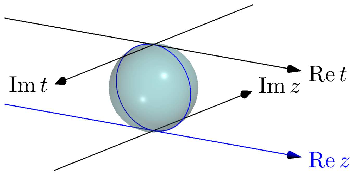
\includegraphics{3dfigures/pdf/Cinf.pdf}
\end{center}
As before, we let $z$ and $t$ parametrize the points on the surface, with $t = \frac{1}{z}$ wherever
both are defined.

Still, we need two dimensions to embed a circle. So, the real part of $\CC \times \CC_\infty$ may
looks something like the following:
\begin{center}
	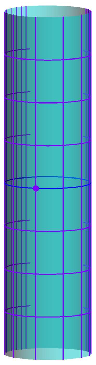
\includegraphics{3dfigures/pdf/CxCinf.pdf}
\end{center}

The grid lines are drawn, and the origin $z = 0$, is marked with a dot.
The vertical lines mark the position $z = 0$, $z = \frac{1}{2}$, $z = 1$, $z = \frac{3}{2}$, \dots.

On the opposite side, we may have something like the following.
The vertical lines mark the position $t = 0$, $t = \frac{1}{2}$, $t = 1$, $t = \frac{3}{2}$, \dots.
\begin{center}
	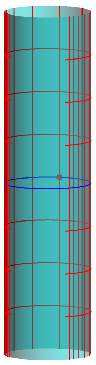
\includegraphics{3dfigures/pdf/CxCinf2.pdf}
\end{center}

\begin{ques}
	Check that, on $\CC \times U$ for any open set $U \subseteq \CC_\infty$ that contains neither
	$0$ nor $\infty$, the two line bundle charts above define the same line bundle structure.
	(What are the transition functions?)
\end{ques}

So, we have the so-called trivial line bundle $\CC \times \CC_\infty$.

As promised, there are also nontrivial line bundles here.

First, recall from the section above: over any open set $U$ that contains neither $0$ nor $\infty$,
we can consider another line bundle chart that scales the vertical direction by a factor of $z$,
this induces the same line bundle structure on $U$.
\begin{center}
\begin{asy}
	size(4cm);
	draw((-5, 0)--(5, 0), blue, Arrow, L=Label("$z$", EndPoint, align=N*1.5+W*0.8));
	draw((0, -5)--(0, 5), Arrow);
	for(int i=-4; i<=4; ++i){
		if(i!=0){
			draw((i, -4.8)--(i, 4.8), purple);
		}
	}
	for(int i=1; i<=4; ++i){
		draw((-4.8,  i)--(i==1 ? 4.2: 4.8, i), purple);
		draw((-4.8, -i)--(4.8, -i), purple);
    }
	for(int i=1; i<=4; ++i){
		draw((-4.8/i, -4.8)--(4.8/i,  4.8), green);
		draw((-4.8/i,  4.8)--(4.8/i, -4.8), green);
    }
\end{asy}
\end{center}
\begin{ques}
	Let $\phi_p$ and $\phi_g$ be the line bundle charts corresponding to the purple and green grid,
	respectively.
	Verify that if a point $q \in L$ satisfies $\phi_p(q) = (y, z)$ for $z \notin \{ 0, \infty \}$,
	then $\phi_g(q) = (\frac{y}{z}, z)$.
\end{ques}
Now --- note that the trivial line bundle $\CC \times \CC_\infty$ above can be seen as welding the
two pieces together, such that the purple line $(y, z)$ gets welded to the red line $(y, t)$ for each
$y$.
There is nothing that restricts us to that specific welding method, however --- this time around, we
will try to weld the green line $(\frac{y}{z}, z)$ to the red line $(y, t)$ for each $y$.

The thing will look like this. It looks quite complicated, so this time 4 views are shown.
\begin{center}
	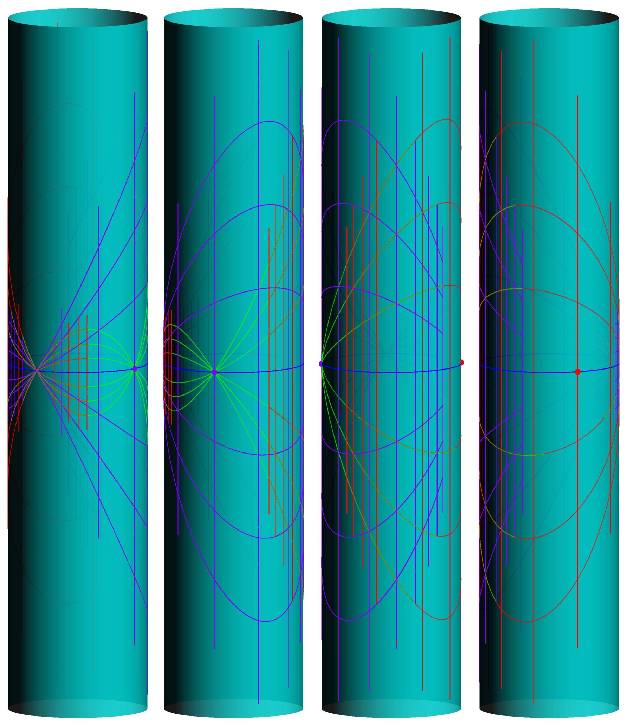
\includegraphics{3dfigures/pdf/CxCinf3.pdf}
\end{center}

The cylinder this time is only for illustrative purpose. Let us see what is going on.
\begin{itemize}
	\ii First, near the purple and the red point, the graph lines looks like our usual situation.

	Note that because $t = \frac{1}{z}$, looking from outside, the red coordinate lines will looks
	flipped.
	\ii On the positive side ($z > 0$ and $t > 0$), no problem --- we just need to squeeze the
	purple lines closer together --- as depicted in the figure.
	\ii On the negative side, however --- note that the green line $(\frac{y}{z}, z)$ moves
	\emph{downwards} when $y$ increases, so we will need to ``twist the graph paper'' for it to go
	up.

	In the figure, this is depicted as a singularity where all the horizontal lines intersect, but
	in reality, you should think of it as we twisting the ``graph paper'' by 180 degrees
	and weld it to the other part.
\end{itemize}

This is a M\"obius strip!

Thus, it appears to be obvious that this line bundle is not isomorphic to the trivial one,
whatever ``isomorphic'' might mean.

\begin{ques}
	Check that what we did above makes sense when $y$, $z$ and $t$ are not real --- in particular,
	$\CC \setminus \{ 0 \}$ is a connected set, unlike $\RR \setminus \{ 0 \}$.
	You probably won't be able to visualize the ``graph paper'' this time (it is
	$4$-dimensional!), so you will have to keep your intuition confined in the real part and use
	algebra for the rest.
\end{ques}

\section{Morphisms between line bundles}

In order to formally define what it means for two line bundles to be isomorphic, we need to be able
to define morphisms.
It is exactly what you expect --- it must respect the line bundle structure (that is, the vector
space structure and the analytic structure) on $L_1$ and $L_2$.

\begin{definition}
	Let $\pi_1 \colon L_1 \to X$ and $\pi_2 \colon L_2 \to X$ be line bundles.
	A line bundle morphism $\alpha \colon L_1 \to L_2$ is a set morphism such that:
	\begin{itemize}
		\ii $\pi_2 \circ \alpha = \pi_1$, and
		\ii if $\phi_1 \colon \pi_1\inv(U_1) \to \CC \times U_1$
		and $\phi_2 \colon \pi_2\inv(U_2) \to \CC \times U_2$
		are line bundle charts, then the composition
		\[ \phi_2 \circ \alpha \circ \phi_1\inv \colon
			\CC \times (U_1 \cap U_2) \to \CC \times (U_1 \cap U_2) \]
		has the form $(s, p) \mapsto (f(p) \cdot s, p)$ where $f$ is analytic on $U_1 \cap U_2$.
	\end{itemize}
\end{definition}

\begin{exercise}
	The function $f(p)$ above must be nonzero for all $p \in U_1 \cap U_2$. Why? (Hint: invert the
	function by swapping the role of $\phi_1$ and $\phi_2$.)
\end{exercise}

\begin{ques}
	Check that the above definition is the equivalent to the following:
	$\alpha$ is a line bundle morphism if and only if
	\begin{itemize}
		\ii it maps a point $q \in \pi_1\inv(x)$ to some point $\alpha(q) \in \pi_2\inv(x)$ (that
		is, each fiber gets mapped to the corresponding fiber), and
		\ii for every analytic section $s \colon U \to L_1$ on open set $U \subseteq X$, then
		$\alpha(s)$ is an analytic section $s \colon U \to L_2$.
	\end{itemize}
\end{ques}

\begin{example}
	Let $X = \CC$. Then $\alpha \colon \CC \times X \to \CC \times X$ by $\alpha(y, x) =
	(y \cdot x^2, x)$ is a line bundle homomorphism.

	This line bundle homomorphism is not an isomorphism, because every point $(y, 0)$ gets mapped to
	$(0, 0)$.
\end{example}

The definition of line bundle isomorphism is what you would expect.
\begin{definition}[Isomorphism of line bundles]
	Two line bundles $L_1$ and $L_2$ are \vocab{isomorphic} if there are line bundle isomorphisms
	$\alpha \colon L_1 \to L_2$ and $\beta \colon L_2 \to L_1$ that are inverse of each other.
\end{definition}

\section{Relation to invertible sheaves}
\todo{write (actually we haven't defined sheaf yet either)}
